%! app: regular-languages, context-free-languages
%! outcome: Formal definition of automata, Informal definition of automata, Nondeterminism, Classify language, Find example languages

Consider the state diagram of a PDA with input alphabet 
$\Sigma$ and stack alphabet $\Gamma$.

\vspace{-0.2in}

\begin{center}
\begin{tabular}{|c|c|}
\hline
Label & means \\
\hline
$a, b \to c$ when $a \in \Sigma$, $b\in \Gamma$, $c \in \Gamma$ 
& \hspace{3in} \\
& \\
&\\
\hline
$a, \varepsilon \to c$ when $a \in \Sigma$, $c \in \Gamma$ 
& \hspace{3in} \\
& \\
&\\
\hline
$a, b \to \varepsilon$ when $a \in \Sigma$, $b\in \Gamma$
& \hspace{3in} \\
& \\
&\\
\hline
$a, \varepsilon \to \varepsilon$ when $a \in \Sigma$
& \hspace{3in} \\
& \\
&\\
\hline
\end{tabular}
\end{center}

\vspace{-0.2in}

How does the meaning change if $a$ is replaced by $\varepsilon$?


For the PDA state diagrams below, $\Sigma = \{0,1\}$.


\vspace{-0.2in}


\begin{center}
\begin{tabular}{c c}
Mathematical description of language & State diagram of PDA recognizing language\\
\hline
& 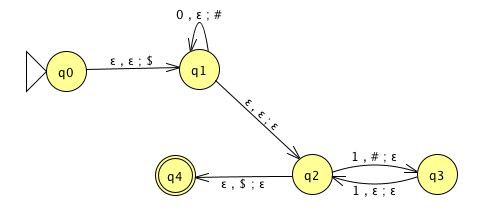
\includegraphics[width=3.5in]{../../resources/machines/Lect10PDA1.png}\\
\hline
& 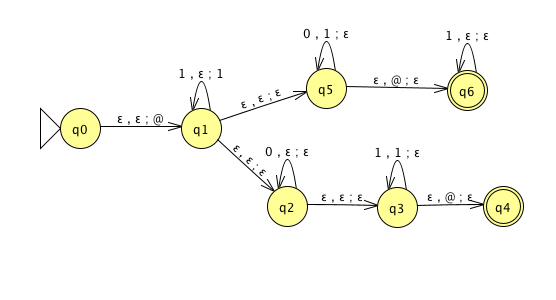
\includegraphics[width=3.5in]{../../resources/machines/Lect10PDA2.png}\\
\hline
& \\
$\{ 0^i 1^j 0^k \mid i,j,k \geq 0 \}$ & \\
\end{tabular}
\end{center}

\newpage

Assume $a \in \Sigma$ and $L$ is a language over $\Sigma$.  Recall that 
\[
aL = \{ aw \mid w \in L \}
\]
If $M = (Q, \Sigma, \Gamma, \delta, q_0, F)$ is a PDA with $L(M) = L$, 
a PDA $M_1$ that recognizes $aL$ is
\[
M_1 = ( \hspace{1in} , \Sigma, \Gamma, \delta_1, \hspace{0.5in}, \hspace{0.5in})
\]
with

\vspace{180pt}

